\section{Requirements of a Web Mapping Pipeline}
\label{sec:introduction:web:mapping:pipelines}

\begin{figure}[htbp]
\begin{center}
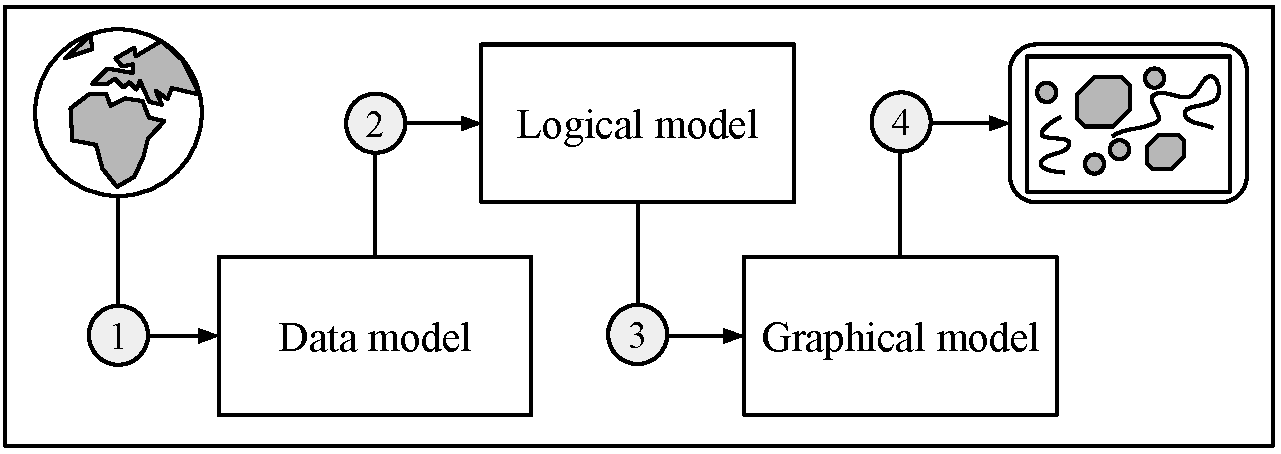
\includegraphics[scale=.5]{figs-thesis/mapping-states.pdf}
\caption{\textbf{States and transitions of a digital mapping pipeline}: data modelling (1); logical abstraction (2); graphical abstraction (3); rendering (4).}
\label{fig:introduction:requirements:pipeline}
\end{center}
\vspace*{-4ex}
\end{figure}

The digital mapping process can be modelled as a pipeline that translates between ``reality'' and a configuration of pixels on a computer screen, i.e. the digital map. This mapping pipeline has three intermediate states that correspond to increasingly abstract representations of reality. These intermediate states are: the \emph{data model}, the \emph{logical model} and the \emph{graphical model} of the digital map~\cite{gruenreich1992atkis} (see Figure~\ref{fig:introduction:requirements:pipeline}).

While the final state is reached by a straight-forward rendering of the graphical model, the three intermediate states and their connecting transitions require further explanation:

\begin{enumerate}
\item \textbf{Data model}: the data model behind a map captures reality as a set of discrete geographic information objects. Geographic information objects associate a \emph{geometry}, such as a point, line or area, with a set of \emph{qualitative}, \emph{ordered} and/or \emph{quantitative components}~\cite{bertin1967semiologie}.
\item \textbf{Logical model}: the logical model of a map logically abstracts the data model by \emph{selection}, \emph{projection} and \emph{aggregration} of the geographic information objects, in order to emphasize the important and suppress the irrelevant. The logical model captures what information the digital map \emph{contains}, but not how it is \emph{displayed}. It should be noted that here the term projection is used as it is used in databases, i.e. the denote modification of an information object.
\item \textbf{Graphical model}: the graphical model of a map graphically abstracts the logical model into a set of symbols, such that the conditions for efficient \emph{visual perception} and \emph{comprehension} in the digital map are maximized. Symbols use \emph{size}, \emph{value}, \emph{texture}, \emph{color}, \emph{orientation}, and \emph{shape} to express the \emph{qualitative}, \emph{ordered} and \emph{quantitative} components of the geographic information~\cite{bertin1967semiologie}. The symbols are arranged according to the geometries of the geographic information objects, either by a strict geometric projection into the plane or in a topologically equivalent arrangement. The graphic model captures \emph{how} the information should be visually represented on a digital map.
\end{enumerate}

There is an important interplay between the logical and graphical model. Different graphical abstractions may trigger the need for new logical abstractions, even through the graphical abstraction step is downstream from the logical abstraction step in Figure~\ref{fig:introduction:requirements:pipeline}. For example, choosing symbols of larger size in the graphical model means that information objects are more likely to overlap. This in turn may requires a renewal of the logical model, such that objects are selected that are futher apart. In conclusion, the ordering of these two states is somewhat arbitrary, and can be sensibly modeled either way.

Research must study the requirements of the mapping pipeline, since this allows researchers to compare state-of-the-art pipelines against hypothetical pipelines that meets all of the requirements. Naturally, mapping pipelines have been studied extensively in the literature. Transition one (data modeling) has been studied in previous work by Friis-Christensen~\cite{friis2001requirements} and Goodchild~\cite{goodchild1992geographical}; Transition three (graphical abstraction) has been studied in the seminal work by Bertin~\cite{bertin1967semiologie}. Transition four (rendering of symbols) is fairly straight-forward and will not be discussed further. This thesis will focus on transition two (logical abstraction), since the biggest challenges in web mapping are currently found here. The requirements for this step are discussed in Section~\ref{sec:introduction:requirements:logical:abstraction}.

The above view of a mapping pipeline is agnostic of the existence of the Web or the Internet. In contrast, a \emph{web mapping pipeline} requires the transfer of state over the Internet, from one state container to another state container. Typically, one state container (the server) transfers state to many state containers (the clients). It is important to understand the requirements of state transfer on the Web and over the Internet. These requirements are discussed in Section~\ref{sec:introduction:requirements:distribution}.

\subsection{Selection} 
\label{sec:introduction:requirements:logical:abstraction}

A smaller scale map implies that less graphical real-estate is available to represent more geographical information. Consequently, information must be omitted by selection, adjusted by projection, or combined by aggregation, which is the process of logical abstraction. This section discusses the constraints and objectives that drive logical abstraction. In doing so, this thesis implicitely adopts a \emph{combinatorial optimization} view of the map generalisation process~\cite{harrie2007modelling}. Furthermore, this thesis focuses on selection as the means for logical abstraction of information. In contrast to selection in relational algebra, selection of geographic information is a holistic process, which cannot be satisfied by filtering the information objects by unary predicates alone~\cite{harrie2007modelling}. 

Even as the Web has impacted when, why and how maps are created and consumed, information that is displayed on maps must (still) be legible, consistent with reality, and relevant for the purpose of the map. This can be ensured by constraints and objectives. 

\begin{ex}[iOS6 Apple Maps Design Goals]
\label{ex:ios6:design:goals}
The iOS6 Apple Maps API fullfils six design goals, which concretize the high-level goals of maps. They express conditions that can be reached by selection, projection and aggregation of geographic information, and therefore are goals for the logical map model: 

\begin{enumerate}
\item minimize overlaps
\item respect relative importance of entries
\item maximize spatial fullness
\item provide panning/zooming consistency
\item enable efficient sampling
\item support filtering conditions
\end{enumerate}
\end{ex}


While Example~\ref{ex:ios6:design:goals} is illustrative of the design goals that drive logical abstraction, a goal of this thesis is to derive a more formal classification of constraints and objectives for logical abstraction of geographic information: 

\begin{itemize}

\item \textbf{Constraints}, namely unary~\cite{de2004simplifying,welch1982spatial}, binary~\cite{nutanong2012multiresolution}, space~\cite{topfer1966principles, woodruff1998constant}, cross-scale~\cite{sarma2012fusiontables,foerster2010challenges} and topological~\cite{egenhofer1991categorizing,randell1992spatial,schmid2013opensciencemap,shreve1966statistical,van1995gap} constraints, define the feasible states of a map. As such, constraints define a search space of feasible maps that are candidates for a logical model. Objects or spaces that violate the constraints are said to be \emph{in conflict}, which is a situation that must be remedied by the application of an appropriate map generalization operator, such as selection~\cite{shea1989cartographic,weibel1997generalization}. These constraint classes, except unary constraints, are holistic since they generally take the entire information set into account when evaluating whether any given object or space is in conflict.

\item \textbf{Objectives}, such as minimization of conflict~\cite{bader2001energy,haunert2006landcover,sester2000generalization} or maximization of relevance~\cite{sarma2012fusiontables,nutanong2012multiresolution}, quantify the utility of a map. Numeric objective functions facilitate combinatorial optimization over the search space of feasible maps. 

\end{itemize}

Given an initial map state, typically corresponding to the primary data model, different logical models can be derived by the application of map generalization operators, i.e. selection, projection and aggregation. Each derived state may be evaluated against the constraints and objectives, in order to decide its feasibility and utility. According to combinatorial optimization view of map generalization, the derived logical model for a map must satisfy the active constraints and be optimal with regard to the objective. These are the core requirements of logical abstraction that are considered by this thesis.


\subsection{Distribution} 
\label{sec:introduction:requirements:distribution}
In stage four of the web mapping pipeline, map content is distributed over the Internet to web and mobile mapping clients. The success criteria are established in a service level aggrements (SLA), which states the acceptable thresholds of quantifiable service metrics. While SLAs differ in their formulation, usually, acceptable thresholds for the following three metrics are defined:

\begin{itemize}
\item \textbf{Availability} is the property that geographic information can be reached and downloaded by mapping client. It can be quantified in terms of so-called ``nines''. For example, ``two nines'' equals 99\% availability or 1.68 hours of downtime per week, while ``five nines'' equals 99.999\% availability or 6.05 seconds of downtime per week. In the EU, national mapping agencies are typically obligated to met at most ``three nines'' of availability~\cite{gst2014digitalmapsupply}. In contrast, private corporations -- such as Google and Microsoft -- rutinely operate at ``four nines'' or ``five nines''. As online map users have come to expect the relative high availability of commecial map distributions, national mapping agencies are presented with a challenge.

\item \textbf{Performance} is the property that requests for geographic information can be evaluated with low latency, which is quantified as the number of milliseconds that a request may take to complete. Studies have shown that user satisfaction is highly sensitive to high -- as well as variation in -- latency~\cite{hamilton2009costoflatency}.

\item \textbf{Scalability} is the property that operational levels, such as acceptable latency, can be sustained for increasing values of some fundamental quantity, typically data volume or concurrency level. To be truely scalable, an architecture must be able to scale with a sub-proportional increase in cost~\cite{vogels2006podcast}.

\end{itemize}

Keeping down the cost is one of the most critical challenges for map content distribution with sustained high availability and acceptable latency. Partitioning of data into\emph{Vector tiles} is an important technique for reaching these goals~\cite{gaffuri12vectortiles}. In this type of distribution, stage three of the pipeline executes on mapping clients. Essentialy, mapping clients contribute processing power to the pipeline rather than only consume it, which consequently makes the pipeline more scalable. In addition, the data partitioning itself facilitates high availability, scalability and performance.
